\chapter{Exercise 1}

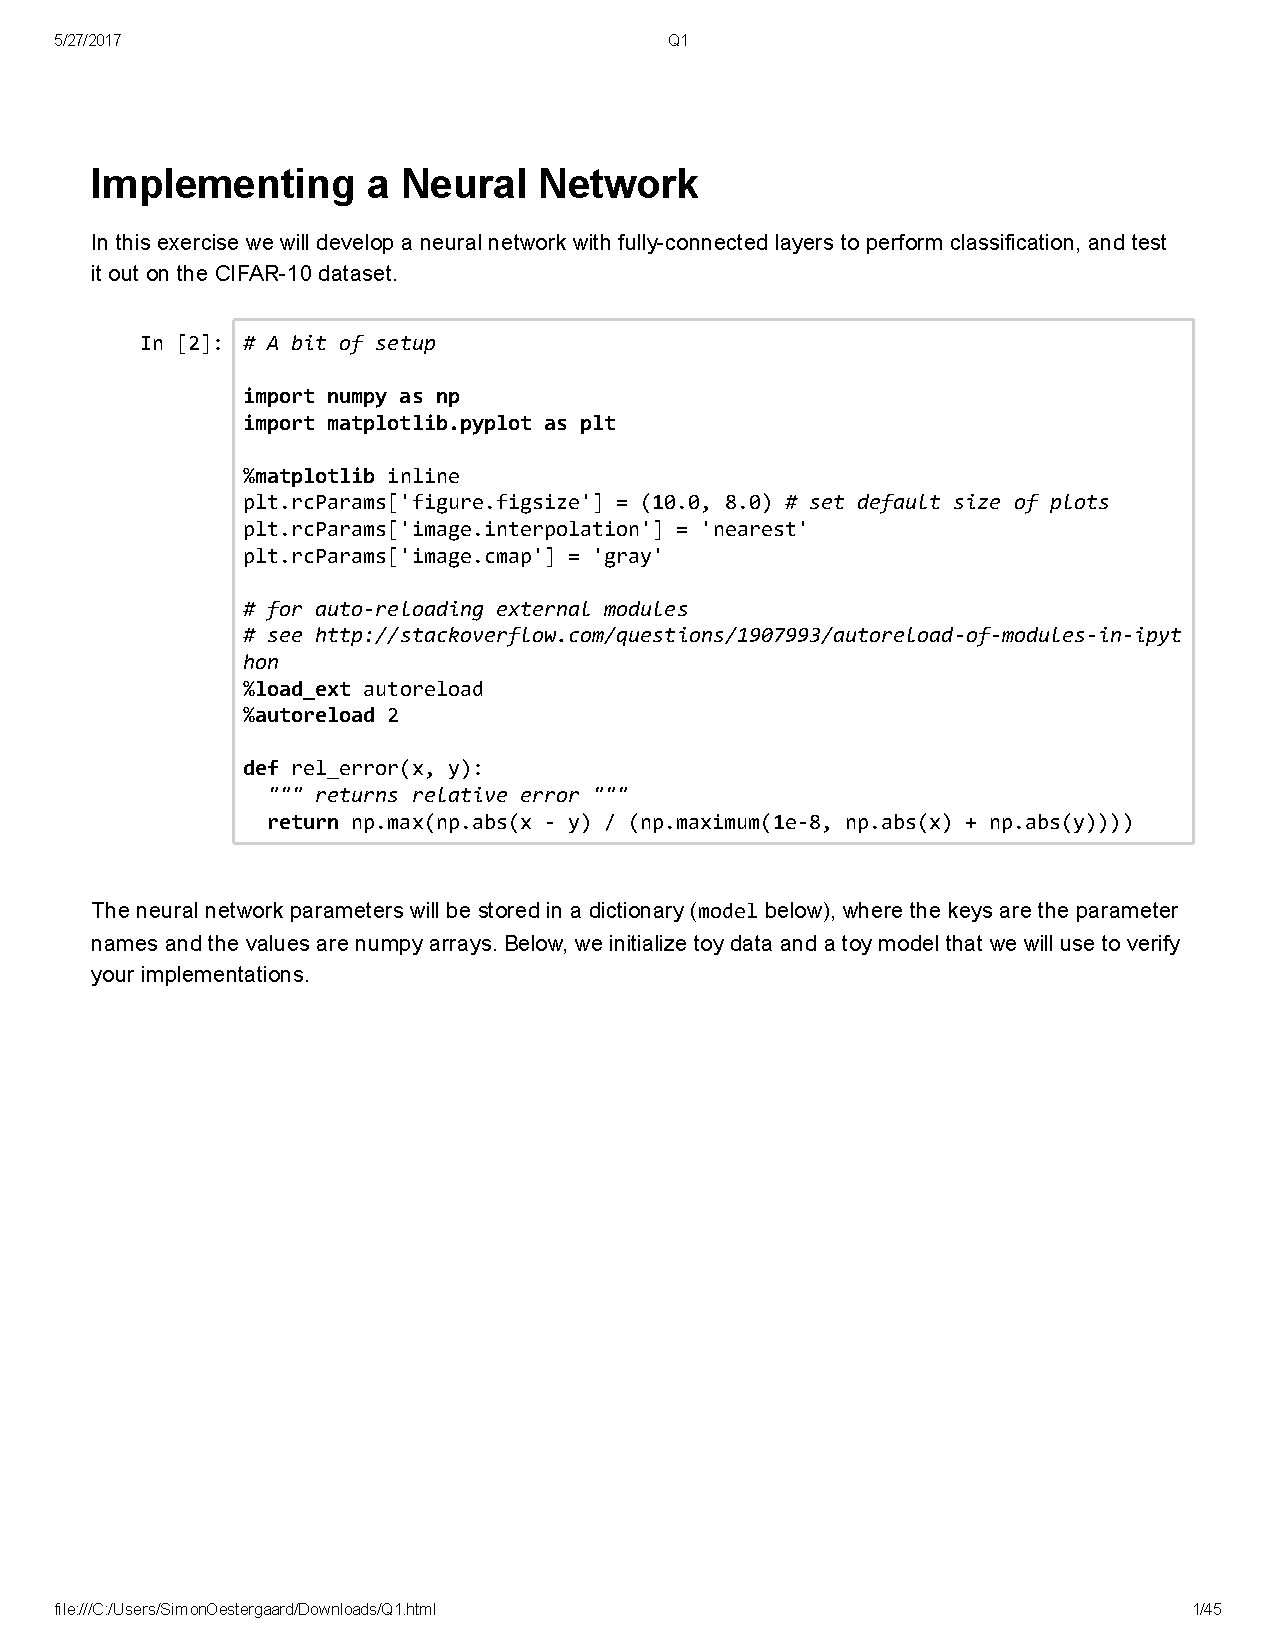
\includepdf[pages={-20}]{chapter/Q1.pdf}
\includepdf[pages={44-}]{chapter/Q1.pdf}
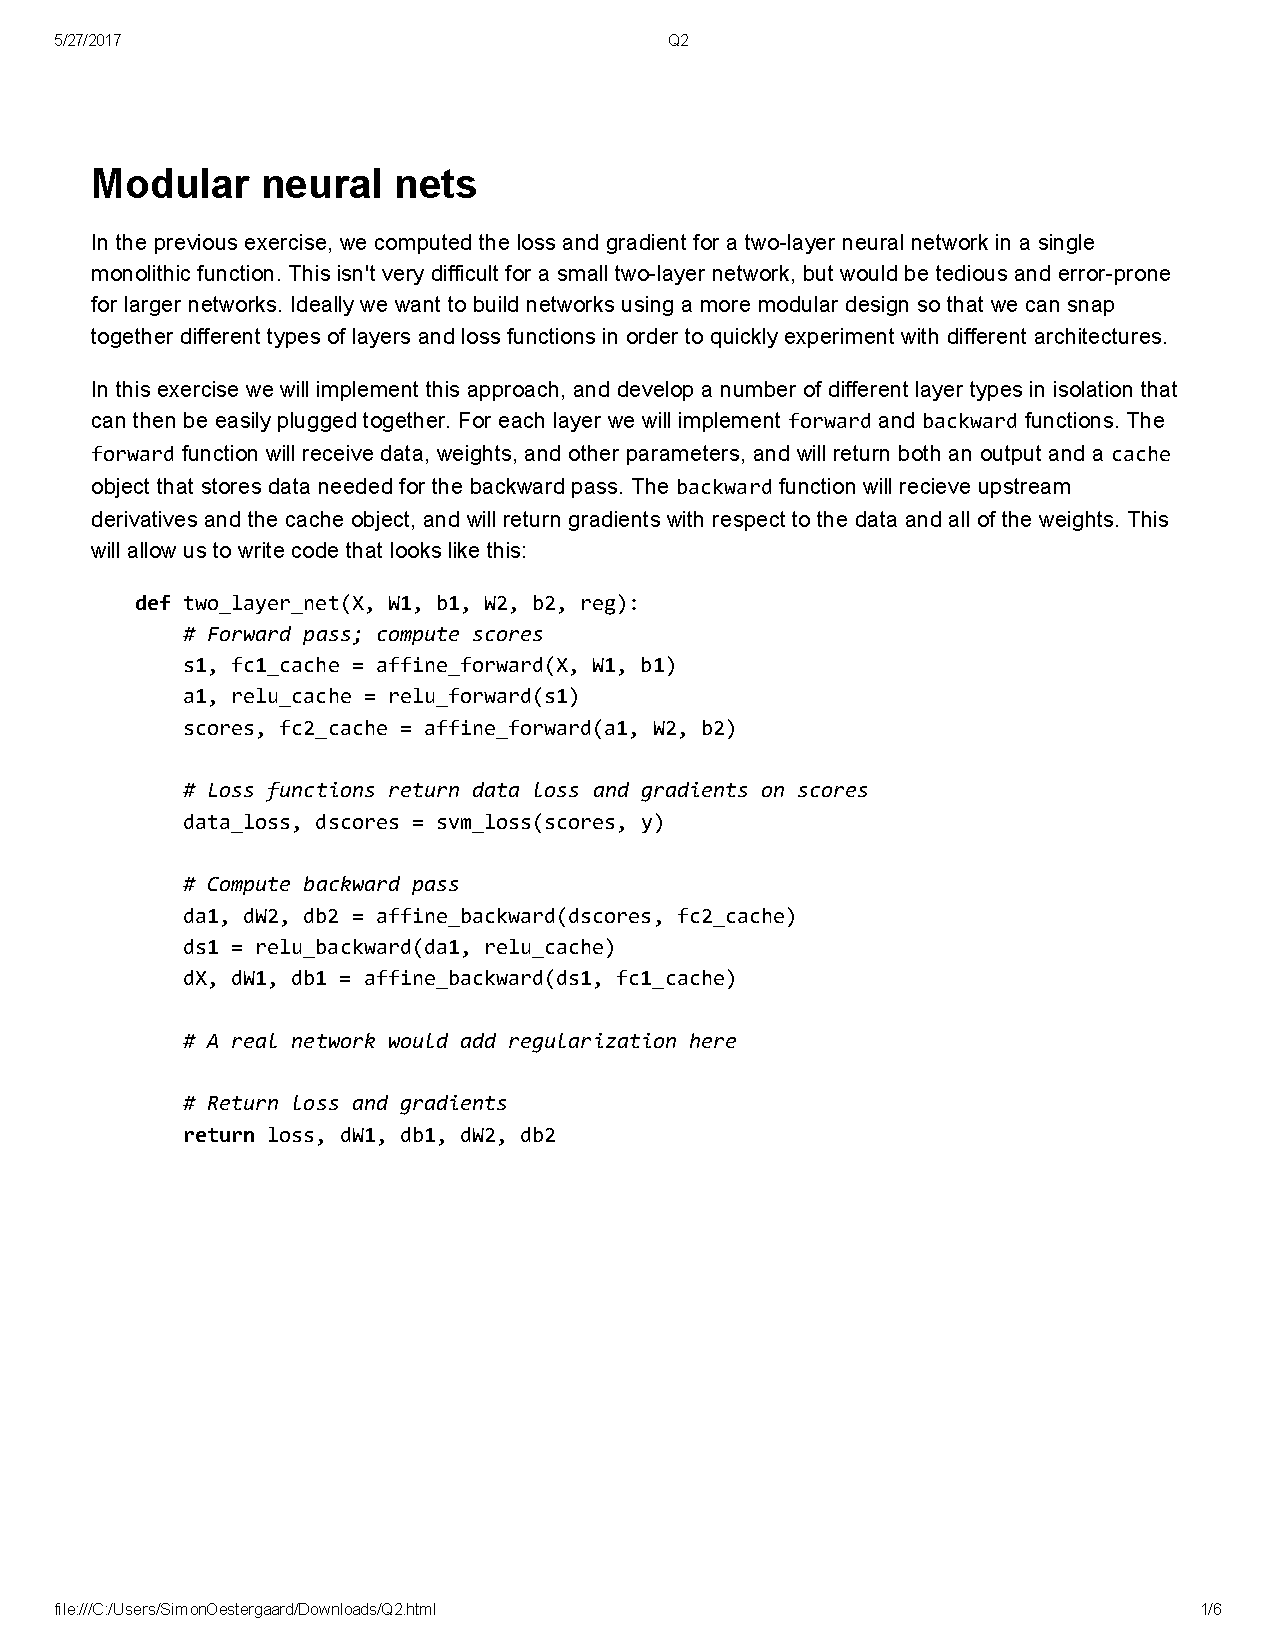
\includepdf[pages={-}]{chapter/Q2.pdf}





\begin{lstlisting}[language=Python, label=lst:neuralnet.py, caption={neural\_net.py}, basicstyle=\tiny]
import numpy as np
import matplotlib.pyplot as plt

def init_two_layer_model(input_size, hidden_size, output_size):
"""
Initialize the weights and biases for a two-layer fully connected neural
network. The net has an input dimension of D, a hidden layer dimension of H,
and performs classification over C classes. Weights are initialized to small
random values and biases are initialized to zero.

Inputs:
- input_size: The dimension D of the input data
- hidden_size: The number of neurons H in the hidden layer
- ouput_size: The number of classes C

Returns:
A dictionary mapping parameter names to arrays of parameter values. It has
the following keys:
- W1: First layer weights; has shape (D, H)
- b1: First layer biases; has shape (H,)
- W2: Second layer weights; has shape (H, C)
- b2: Second layer biases; has shape (C,)
"""
# initialize a model
model = {}
model['W1'] = 0.00001 * np.random.randn(input_size, hidden_size)
model['b1'] = np.zeros(hidden_size)
model['W2'] = 0.00001 * np.random.randn(hidden_size, output_size)
model['b2'] = np.zeros(output_size)
return model

def two_layer_net(X, model, y=None, reg=0.0):
"""
Compute the loss and gradients for a two layer fully connected neural network.
The net has an input dimension of D, a hidden layer dimension of H, and
performs classification over C classes. We use a softmax loss function and L2
regularization the the weight matrices. The two layer net should use a ReLU
nonlinearity after the first affine layer.

The two layer net has the following architecture:

input - fully connected layer - ReLU - fully connected layer - softmax

The outputs of the second fully-connected layer are the scores for each
class.

Inputs:
- X: Input data of shape (N, D). Each X[i] is a training sample.
- model: Dictionary mapping parameter names to arrays of parameter values.
It should contain the following:
- W1: First layer weights; has shape (D, H)
- b1: First layer biases; has shape (H,)
- W2: Second layer weights; has shape (H, C)
- b2: Second layer biases; has shape (C,)
- y: Vector of training labels. y[i] is the label for X[i], and each y[i] is
an integer in the range 0 <= y[i] < C. This parameter is optional; if it
is not passed then we only return scores, and if it is passed then we
instead return the loss and gradients.
- reg: Regularization strength.

Returns:
If y not is passed, return a matrix scores of shape (N, C) where scores[i, c]
is the score for class c on input X[i].

If y is not passed, instead return a tuple of:
- loss: Loss (data loss and regularization loss) for this batch of training
samples.
- grads: Dictionary mapping parameter names to gradients of those parameters
with respect to the loss function. This should have the same keys as model.
"""

# unpack variables from the model dictionary
W1,b1,W2,b2 = model['W1'], model['b1'], model['W2'], model['b2']
N, D = X.shape  
# input - fully connected layer - ReLU - fully connected layer - softmax
#Activation function
reluF = lambda x: np.maximum(0, x)
#Compared to lecture notes we switch X and W1 because to multiple the inputs 
#with the correct weights
h1 = reluF(np.dot(X, W1) + b1)
scores = np.dot(h1, W2) + b2
#############################################################################
#                              END OF YOUR CODE                             #
#############################################################################

# If the targets are not given then jump out, we're done
if y is None:
return scores

#############################################################################
# TODO: Finish the forward pass, and compute the loss. This should include  #
# both the data loss and L2 regularization for W1 and W2. Store the result  #
# in the variable loss, which should be a scalar. Use the Softmax           #
# classifier loss. So that your results match ours, multiply the            #
# regularization loss by 0.5                                                #
#############################################################################
# compute the loss
expScores = np.exp(scores)
rowSum = expScores.sum(axis=1, keepdims=True)
# Normalized scores
propScores = expScores / rowSum
logprob_correctLabel = -np.log(propScores[range(N),y])
softmax_loss = 1/float(N) * np.sum(logprob_correctLabel)
#regulization loss
reg_loss = 0.5 * reg * np.sum(W1*W1) + 0.5 * reg * np.sum(W2 * W2)
#Final loss 
loss = softmax_loss + reg_loss
#############################################################################
#                              END OF YOUR CODE                             #
#############################################################################

# compute the gradients
grads = {}

#############################################################################
# TODO: Compute the backward pass, computing the derivatives of the weights #
# and biases. Store the results in the grads dictionary. For example,       #
# grads['W1'] should store the gradient on W1, and be a matrix of same size #
#############################################################################
# Firstly we calculate the gradient on the scores.
# The gradient from the loss function is simply -1.
# This is subtracted from the correct scores for each
# dscores are the probabilities for all classes as a row for each sample
dscores = propScores
#For each row(sample) in dscores 1 is subtracted from the correct element 
#specified by y
dscores[range(N),y] -= 1
# We then divide all elements with N(number of samples)
dscores /= N

# The gradient for W2 is simply the output from the RELU activation function (h1)
# multiplyed with the dscores that contains the gradient on the scores.
# d/dw(w*x) = x which is our h1 then we get the input times dscores
grads['W2'] = np.dot(h1.T, dscores)
#bias is just the sum of the dscores
grads['b2'] = np.sum(dscores, axis=0)

# next backprop into hidden layer. This is the scores multiplied with the weights
# for second layer
dhidden = np.dot(dscores, W2.T)
# backprop the ReLU non-linearity. 
#For elements < or equals 0  we set them equals to 0
# remember how Relu is just max, so it routes the gradients
dhidden[h1 <= 0] = 0
# same thing as second layer - d/dw(w*x) = x, so x times our gradient for dhidden
grads['W1'] = np.dot(X.T, dhidden)
grads['b1'] = np.sum(dhidden, axis=0)

# adding gradient for regulization
# d/dw(1/2*reg*W1*w1) = reg * W1
grads['W1'] += reg * W1 
grads['W2'] += reg * W2
#############################################################################
#                              END OF YOUR CODE                             #
#############################################################################

return loss, grads
\end{lstlisting}










\begin{lstlisting}[language=Python, label=lst:classifiertrainer.py, caption={classifier\_trainer.py}, basicstyle=\tiny]
import numpy as np


class ClassifierTrainer(object):
""" The trainer class performs SGD with momentum on a cost function """
def __init__(self):
self.step_cache = {} # for storing velocities in momentum update

def train(self, X, y, X_val, y_val, 
model, loss_function, 
reg=0.0,
learning_rate=1e-2, momentum=0, learning_rate_decay=0.95,
update='momentum', sample_batches=True,
num_epochs=30, batch_size=100, acc_frequency=None,
verbose=False):
"""
Optimize the parameters of a model to minimize a loss function. We use
training data X and y to compute the loss and gradients, and periodically
check the accuracy on the validation set.

Inputs:
- X: Array of training data; each X[i] is a training sample.
- y: Vector of training labels; y[i] gives the label for X[i].
- X_val: Array of validation data
- y_val: Vector of validation labels
- model: Dictionary that maps parameter names to parameter values. Each
parameter value is a numpy array.
- loss_function: A function that can be called in the following ways:
scores = loss_function(X, model, reg=reg)
loss, grads = loss_function(X, model, y, reg=reg)
- reg: Regularization strength. This will be passed to the loss function.
- learning_rate: Initial learning rate to use.
- momentum: Parameter to use for momentum updates.
- learning_rate_decay: The learning rate is multiplied by this after each
epoch.
- update: The update rule to use. One of 'sgd', 'momentum', or 'rmsprop'.
- sample_batches: If True, use a minibatch of data for each parameter update
(stochastic gradient descent); if False, use the entire training set for
each parameter update (gradient descent).
- num_epochs: The number of epochs to take over the training data.
- batch_size: The number of training samples to use at each iteration.
- acc_frequency: If set to an integer, we compute the training and
validation set error after every acc_frequency iterations.
- verbose: If True, print status after each epoch.

Returns a tuple of:
- best_model: The model that got the highest validation accuracy during
training.
- loss_history: List containing the value of the loss function at each
iteration.
- train_acc_history: List storing the training set accuracy at each epoch.
- val_acc_history: List storing the validation set accuracy at each epoch.
"""

N = X.shape[0]

if sample_batches:
iterations_per_epoch = N / batch_size # using SGD
else:
iterations_per_epoch = 1 # using GD
num_iters = num_epochs * iterations_per_epoch
epoch = 0
best_val_acc = 0.0
best_model = {}
loss_history = []
train_acc_history = []
val_acc_history = []
for it in xrange(num_iters):
if it % 10 == 0:  print 'starting iteration ', it

# get batch of data
if sample_batches:
batch_mask = np.random.choice(N, batch_size)
X_batch = X[batch_mask]
y_batch = y[batch_mask]
else:
# no SGD used, full gradient descent
X_batch = X
y_batch = y

# evaluate cost and gradient
cost, grads = loss_function(X_batch, model, y_batch, reg)
loss_history.append(cost)

# perform a parameter update
for p in model:
# compute the parameter step
if update == 'sgd':
dx = -learning_rate * grads[p]
elif update == 'momentum':
if not p in self.step_cache: 
self.step_cache[p] = np.zeros(grads[p].shape)
dx = np.zeros_like(grads[p]) # you can remove this after
#####################################################################
# TODO: implement the momentum update formula and store the step    #
# update into variable dx. You should use the variable              #
# step_cache[p] and the momentum strength is stored in momentum.    #
# Don't forget to also update the step_cache[p].                    #
#####################################################################
# Momentum update
# Momentum strength is a coefficient explains to friction,
# moment strength damps velocity and reduces the kinetic energy
#it ensures that the particle stops at the bottom
# step_cache is our velocity at time t-1
# From that we subtract the learning rate multiplied the gradients, 
# because we go in the opposite direction of the gradient
dx = momentum * self.step_cache[p] - learning_rate * grads[p] # integrate velocity
self.step_cache[p] = dx 

#####################################################################
#                      END OF YOUR CODE                             #
#####################################################################
elif update == 'rmsprop':
decay_rate = 0.99 # you could also make this an option
if not p in self.step_cache: 
self.step_cache[p] = np.zeros(grads[p].shape)
#####################################################################
# TODO: implement the RMSProp update and store the parameter update #
# dx. Don't forget to also update step_cache[p]. Use smoothing 1e-8 #
#####################################################################
#eps = 1e-8
eps = 1e5
self.step_cache[p] = decay_rate * self.step_cache[p] + (1 - decay_rate) * grads[p]**2
dx = - learning_rate * grads[p] / (np.sqrt(self.step_cache[p]) + eps)


#####################################################################
#                      END OF YOUR CODE                             #
#####################################################################
else:
raise ValueError('Unrecognized update type "%s"' % update)

# update the parameters
model[p] += dx

# every epoch perform an evaluation on the validation set
first_it = (it == 0)
epoch_end = (it + 1) % iterations_per_epoch == 0
acc_check = (acc_frequency is not None and it % acc_frequency == 0)
if first_it or epoch_end or acc_check:
if it > 0 and epoch_end:
# decay the learning rate
learning_rate *= learning_rate_decay
epoch += 1

# evaluate train accuracy
if N > 1000:
train_mask = np.random.choice(N, 1000)
X_train_subset = X[train_mask]
y_train_subset = y[train_mask]
else:
X_train_subset = X
y_train_subset = y
scores_train = loss_function(X_train_subset, model)
y_pred_train = np.argmax(scores_train, axis=1)
train_acc = np.mean(y_pred_train == y_train_subset)
train_acc_history.append(train_acc)

# evaluate val accuracy
scores_val = loss_function(X_val, model)
y_pred_val = np.argmax(scores_val, axis=1)
val_acc = np.mean(y_pred_val ==  y_val)
val_acc_history.append(val_acc)

# keep track of the best model based on validation accuracy
if val_acc > best_val_acc:
# make a copy of the model
best_val_acc = val_acc
best_model = {}
for p in model:
best_model[p] = model[p].copy()

# print progress if needed
if verbose:
print ('Finished epoch %d / %d: cost %f, train: %f, val %f, lr %e'
% (epoch, num_epochs, cost, train_acc, val_acc, learning_rate))

if verbose:
print 'finished optimization. best validation accuracy: %f' % (best_val_acc, )
# return the best model and the training history statistics
return best_model, loss_history, train_acc_history, val_acc_history
\end{lstlisting}









\begin{lstlisting}[language=Python, label=lst:layers.py, caption={layers.py}, basicstyle=\tiny]
import numpy as np

def affine_forward(x, w, b):
"""
Computes the forward pass for an affine (fully-connected) layer.

The input x has shape (N, d_1, ..., d_k) where x[i] is the ith input.
We multiply this against a weight matrix of shape (D, M) where
D = \prod_i d_i

Inputs:
x - Input data, of shape (N, d_1, ..., d_k)
w - Weights, of shape (D, M)
b - Biases, of shape (M,)

Returns a tuple of:
- out: output, of shape (N, M)
- cache: (x, w, b)
"""
out = None
#############################################################################
# TODO: Implement the affine forward pass. Store the result in out. You     #
# will need to reshape the input into rows.                                 #
#############################################################################
# First we reshape X to mulitply it with the incoming weights
# We get column and row size and then reshape
row_size = x.shape[0]
col_size = np.prod(x.shape[1:])
x_reshape = x.reshape(row_size, col_size)
# To execute the forward pass we simply need to multiply the inputs with the weights
out = np.dot(x_reshape, w) + b
#############################################################################
#                             END OF YOUR CODE                              #
#############################################################################
cache = (x, w, b)
return out, cache


def affine_backward(dout, cache):
"""
Computes the backward pass for an affine layer.

Inputs:
- dout: Upstream derivative, of shape (N, M)
- cache: Tuple of:
- x: Input data, of shape (N, d_1, ... d_k)
- w: Weights, of shape (D, M)

Returns a tuple of:
- dx: Gradient with respect to x, of shape (N, d1, ..., d_k)
- dw: Gradient with respect to w, of shape (D, M)
- db: Gradient with respect to b, of shape (M,)
"""
x, w, b = cache
dx, dw, db = None, None, None
#############################################################################
# TODO: Implement the affine backward pass.                                 #
#############################################################################
# First we reshape X to mulitply it with the incoming weights
# We get column and row size and then reshape
row_size = x.shape[0]
col_size = np.prod(x.shape[1:])
x_reshape = x.reshape(row_size, col_size)

# After reshaping we calculate the backward pass

# Gradient with respect to x
# Gradient of x*w with respect to x is simply w, 
# We multiply that with the upstream gradient
dx2 = np.dot(dout, w.T) 
dx = np.reshape(dx2, x.shape)

# Gradient with respect to weights
# Gradient of x*w with respect to w is simply x,
# We multiply that with the upstream gradient
dw = np.dot(x_reshape.T, dout)

# Gradient with respect to bias
# Biases are added so the gradient is simply 1,
# We multiply that with the upstream gradient.
db = np.dot(dout.T, np.ones(row_size))

#############################################################################
#                             END OF YOUR CODE                              #
#############################################################################
return dx, dw, db


def relu_forward(x):
"""
Computes the forward pass for a layer of rectified linear units (ReLUs).

Input:
- x: Inputs, of any shape

Returns a tuple of:
- out: Output, of the same shape as x
- cache: x
"""
out = None
#############################################################################
# TODO: Implement the ReLU forward pass.                                    #
#############################################################################
reluF = lambda x: np.maximum(0, x)
out = reluF(x)
#############################################################################
#                             END OF YOUR CODE                              #
#############################################################################
cache = x
return out, cache


def relu_backward(dout, cache):
"""
Computes the backward pass for a layer of rectified linear units (ReLUs).

Input:
- dout: Upstream derivatives, of any shape
- cache: Input x, of same shape as dout

Returns:
- dx: Gradient with respect to x
"""
dx, x = None, cache
#############################################################################
# TODO: Implement the ReLU backward pass.                                   #
#############################################################################
#reluf function
reluF = lambda x: np.maximum(0, x)

out = reluF(x)
# Reluf is a max gate and so we can think of it as a router of gradients
# the max value is the one that the gradient is routated to
# we simpy set the out value to 1 if the out value is bigger than 0
out[out > 0] = 1

# Multiply out  with upstream gradient, to "route" the gradient
dx = out * dout
#############################################################################
#                             END OF YOUR CODE                              #
#############################################################################
return dx

def dropout_forward(x, dropout_param):
"""
Performs the forward pass for (inverted) dropout.

Inputs:
- x: Input data, of any shape
- dropout_param: A dictionary with the following keys:
- p: Dropout parameter. We keep each neuron output with probability p.
- mode: 'test' or 'train'. If the mode is train, then perform dropout;
if the mode is test, then just return the input.
- seed: Seed for the random number generator. Passing seed makes this
function deterministic, which is needed for gradient checking but not in
real networks.

Outputs:
- out: Array of the same shape as x.
- cache: A tuple (dropout_param, mask). In training mode, mask is the dropout
mask that was used to multiply the input; in test mode, mask is None.
"""
p, mode = dropout_param['p'], dropout_param['mode']
if 'seed' in dropout_param:
np.random.seed(dropout_param['seed'])

mask = None
out = None

if mode == 'train':
###########################################################################
# TODO: Implement the training phase forward pass for inverted dropout.   #
# Store the dropout mask in the mask variable.                            #
###########################################################################
pass
###########################################################################
#                            END OF YOUR CODE                             #
###########################################################################
elif mode == 'test':
###########################################################################
# TODO: Implement the test phase forward pass for inverted dropout.       #
###########################################################################
pass
###########################################################################
#                            END OF YOUR CODE                             #
###########################################################################

cache = (dropout_param, mask)
out = out.astype(x.dtype, copy=False)

return out, cache


def dropout_backward(dout, cache):
"""
Perform the backward pass for (inverted) dropout.

Inputs:
- dout: Upstream derivatives, of any shape
- cache: (dropout_param, mask) from dropout_forward.
"""
dropout_param, mask = cache
mode = dropout_param['mode']
if mode == 'train':
###########################################################################
# TODO: Implement the training phase forward pass for inverted dropout.   #
# Store the dropout mask in the mask variable.                            #
###########################################################################
pass
###########################################################################
#                            END OF YOUR CODE                             #
###########################################################################
elif mode == 'test':
dx = dout
return dx


def conv_forward_naive(x, w, b, conv_param):
"""
A naive implementation of the forward pass for a convolutional layer.

The input consists of N data points, each with C channels, height H and width
W. We convolve each input with F different filters, where each filter spans
all C channels and has height HH and width HH.

Input:
- x: Input data of shape (N, C, H, W)
- w: Filter weights of shape (F, C, HH, WW)
- b: Biases, of shape (F,)
- conv_param: A dictionary with the following keys:
- 'stride': The number of pixels between adjacent receptive fields in the
horizontal and vertical directions.
- 'pad': The number of pixels that will be used to zero-pad the input.

Returns a tuple of:
- out: Output data, of shape (N, F, H', W') where H' and W' are given by
H' = 1 + (H + 2 * pad - HH) / stride
W' = 1 + (W + 2 * pad - WW) / stride
- cache: (x, w, b, conv_param)
"""
out = None
#############################################################################
# TODO: Implement the convolutional forward pass.                           #
# Hint: you can use the function np.pad for padding.                        #
#############################################################################
pass
#############################################################################
#                             END OF YOUR CODE                              #
#############################################################################
cache = (x, w, b, conv_param)
return out, cache


def conv_backward_naive(dout, cache):
"""
A naive implementation of the backward pass for a convolutional layer.

Inputs:
- dout: Upstream derivatives.
- cache: A tuple of (x, w, b, conv_param) as in conv_forward_naive

Returns a tuple of:
- dx: Gradient with respect to x
- dw: Gradient with respect to w
- db: Gradient with respect to b
"""
dx, dw, db = None, None, None
#############################################################################
# TODO: Implement the convolutional backward pass.                          #
#############################################################################
pass
#############################################################################
#                             END OF YOUR CODE                              #
#############################################################################
return dx, dw, db


def max_pool_forward_naive(x, pool_param):
"""
A naive implementation of the forward pass for a max pooling layer.

Inputs:
- x: Input data, of shape (N, C, H, W)
- pool_param: dictionary with the following keys:
- 'pool_height': The height of each pooling region
- 'pool_width': The width of each pooling region
- 'stride': The distance between adjacent pooling regions

Returns a tuple of:
- out: Output data
- cache: (x, pool_param)
"""
out = None
#############################################################################
# TODO: Implement the max pooling forward pass                              #
#############################################################################
pass
#############################################################################
#                             END OF YOUR CODE                              #
#############################################################################
cache = (x, pool_param)
return out, cache


def max_pool_backward_naive(dout, cache):
"""
A naive implementation of the backward pass for a max pooling layer.

Inputs:
- dout: Upstream derivatives
- cache: A tuple of (x, pool_param) as in the forward pass.

Returns:
- dx: Gradient with respect to x
"""
dx = None
#############################################################################
# TODO: Implement the max pooling backward pass                             #
#############################################################################
pass
#############################################################################
#                             END OF YOUR CODE                              #
#############################################################################
return dx


def svm_loss(x, y):
"""
Computes the loss and gradient using for multiclass SVM classification.

Inputs:
- x: Input data, of shape (N, C) where x[i, j] is the score for the jth class
for the ith input.
- y: Vector of labels, of shape (N,) where y[i] is the label for x[i] and
0 <= y[i] < C

Returns a tuple of:
- loss: Scalar giving the loss
- dx: Gradient of the loss with respect to x
"""
N = x.shape[0]
correct_class_scores = x[np.arange(N), y]
margins = np.maximum(0, x - correct_class_scores[:, np.newaxis] + 1.0)
margins[np.arange(N), y] = 0
loss = np.sum(margins) / N
num_pos = np.sum(margins > 0, axis=1)
dx = np.zeros_like(x)
dx[margins > 0] = 1
dx[np.arange(N), y] -= num_pos
dx /= N
return loss, dx


def softmax_loss(x, y):
"""
Computes the loss and gradient for softmax classification.

Inputs:
- x: Input data, of shape (N, C) where x[i, j] is the score for the jth class
for the ith input.
- y: Vector of labels, of shape (N,) where y[i] is the label for x[i] and
0 <= y[i] < C

Returns a tuple of:
- loss: Scalar giving the loss
- dx: Gradient of the loss with respect to x
"""
probs = np.exp(x - np.max(x, axis=1, keepdims=True))
probs /= np.sum(probs, axis=1, keepdims=True)
N = x.shape[0]
loss = -np.sum(np.log(probs[np.arange(N), y])) / N
dx = probs.copy()
dx[np.arange(N), y] -= 1
dx /= N
return loss, dx
\end{lstlisting}